\documentclass[conference]{IEEEtran}
\IEEEoverridecommandlockouts
% The preceding line is only needed to identify funding in the first footnote. If that is unneeded, please comment it out.
\usepackage{cite}
\usepackage{amsmath,amssymb,amsfonts}
\usepackage{algorithmic}
\usepackage{graphicx}
\usepackage[tight,footnotesize]{subfigure}
\usepackage{textcomp}
\usepackage{xcolor}

%for hungarian letters
\usepackage[utf8]{inputenc}

\def\BibTeX{{\rm B\kern-.05em{\sc i\kern-.025em b}\kern-.08em
    T\kern-.1667em\lower.7ex\hbox{E}\kern-.125emX}}


\title{Hindsight Experience Replay with Environment Relabeling \\
	\bigskip
\Large{Milestone Report}}

\author{\IEEEauthorblockN{Katharina Hermann}
	\IEEEauthorblockA{\textit{Technische Universität München}}
	\textit{Department of Informatics}
	\and
	\IEEEauthorblockN{Ferenc Török}
	\IEEEauthorblockA{\textit{Technische Universität München}}
	\textit{Department of Informatics}
}

\begin{document}
\maketitle

\begin{abstract}
	This document is written as a milestone report for the project of the course Advanced Deep Learning in Robotics at the Technische Universität München. Our chosen topic is to develop a method to train a Neural Motin Planner (NMP) \cite{NMP} agent with Reinforcement Learning (RL) \cite{sutton_barto} in an environment with obstacles. The aim of the method is to reduce training time as much as possible meanwhile using a very simple reward function. For this we use Hindsight Experience Replay (HER) \cite{HER, GHER} with environment relabeling. 
\end{abstract}

\section{Experiment Setup}

\textit{Agent}: For now we have used a point-mass robot in 2D for the sake of simplicity. The robot has got a radius. If an obstacle is closer than the radius, a collision occurred. Also, if the goal is within the agent's radius, it is considered to be reached. The agent has 2 continuous actions with which it is able to interact with the environment, a x and y direction step distance. These can be arbitrary values between their respective maximum and minimum values.

\textit{Reward specification}: The task of the agent is to navigate from one point to an other in a workspace which contains some obstacles which should be avoided. Or reward function is as simple as it gets: the agent receives a reward in the amount of $+5$ if the it has reached the goal, $-1$ if it has collided with an obstacle or left the workspace and $-0.01$ after every timestep. 

\textit{Workspace}: Workspaces are represented as a $32 \times 32$ grid, where each grid cell is either free space (value $0$) or obstacle (value$1$). The number of obstacles, their position and size are generated randomly. 

\textit{Start, goal}: Start and goal positions are also generated randomly for a given workspace. A workspace with the obstacles, the goal and the agent is illustrated in Figure \ref{fig:1}.

\textit{Performance metric}: We use success rate as the evaluation metric. In every evaluation cycle, we carry out $N$ evaluation episodes. The succes rate for every evaluation cycle then calculated as follows: $\mu = N_{succ} / N$, where $N_{succ}$ is the number of successful episodes. 

\begin{figure}[h!]
	\centering
	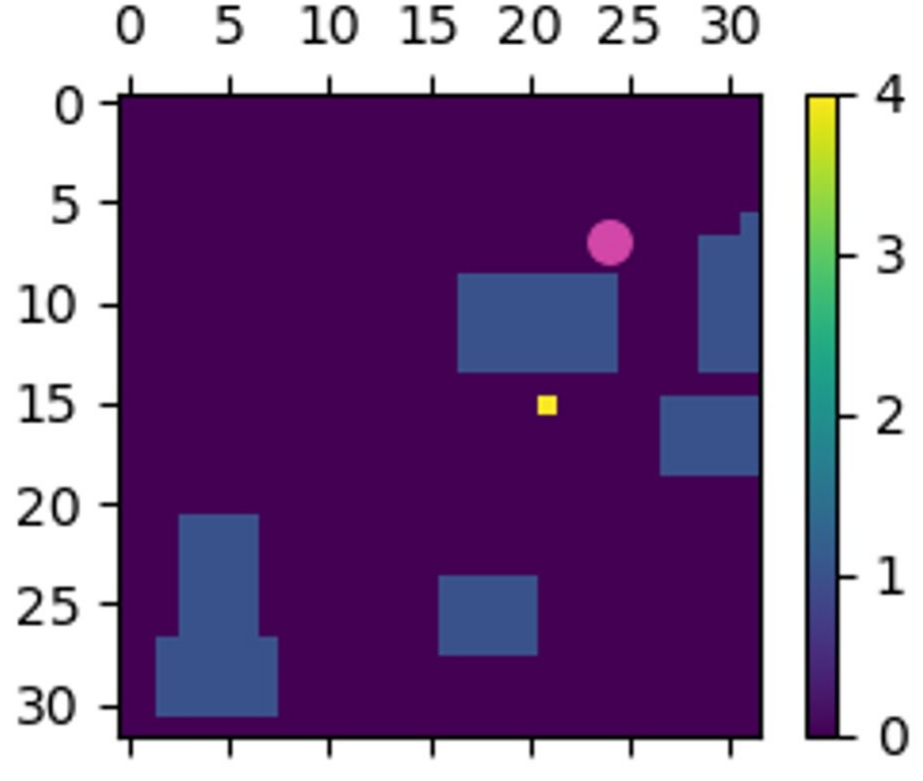
\includegraphics[width=0.2\textwidth]{fig/workspace.jpg}
	\caption{Workspace with obstacles (light blue), agent (pink) and goal (yellow)}
	\label{fig:1}
\end{figure}

\section{Implementation}

We have chosen the agent to be trained with Deep Deterministic Policy Gradient (DDPG) \cite{DDPG} which is an Actor-Critic algorithm for continuous state and action spaces. We use an off-the-shelf implementation, the python package TF2RL \cite{TF2RL}. This package implements various RL methods in Tensorflow 2.x. For the environment we have implemented a custom Open-AI gym environment.

The main building blocks of the project are as follows:
\begin{itemize}
	\item Workspace and goal generation.
	\item Convolutional Autoencoder (CAE) for reducing the workspace representation size. This is necessary since the workspace in its original form is represented with a feature vector of size $1024$. Compared to this, the state of the robot and the goal are represented with $2-2$ features. The workspace feature vector reduction is necessary not to loose the information about the state and the goal position.
	\item Environment implementation as a custom Open-AI gym environment.
	\item Workspace relabeling implementation
	\item Implementation of the trainer class with HER and environment relabeling.
	\item Tests
\end{itemize}

\section{Progress}

So far we have made the following progress:
\begin{itemize}
	\item Implemented and tested workspace, start and goal generation.
	\item Implemented, tested and trained the CAE on $10000$ workspaces. For the encoder we have used 3 Convolutional layers with filter sizes of $[4, 8, 16]$ followed by max-pooling for size reduction. Then after a linear layer the feature size was reduced to the latent space dimension, which is $16$. For the decoding we have used a linear layer followed by transpose convolutional and convolutional layers. We have used weighted binary cross entropy loss for training. With this method we have achieved $96\%$ accuracy on the test set. An example of the original and the output image can be seen on Figure \ref{fig:2}.
	\item Implemented and tested the custome Open-AI gym environment
	\item Implemented and tested a simple relabeling method. The method so far is very simple, it only removes the obstacle into which the agent has collided or shifts the workspace and the trajectory if the agent has left the workspace. The new goal is the last state of the trajectory.
	\item Implemented and tested the training method with HER and workspace relabeling. So far we are looking for good parameters for training. We have trained some agents but the results so far are not sufficient. The actor and critic losses and the training and testing success rates of an experimental training can be seen in Figure \ref{fig:3} and \ref{fig:4} respectively.
\end{itemize}

\begin{figure}[h!]
	\begin{center}
		\subfigure[Input \label{fig:2a}]{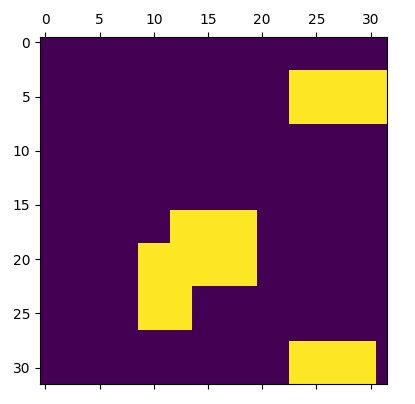
\includegraphics[width=0.2\textwidth]{fig/cae_orig.jpg}}
		~
		\subfigure[Output \label{fig:2b}]{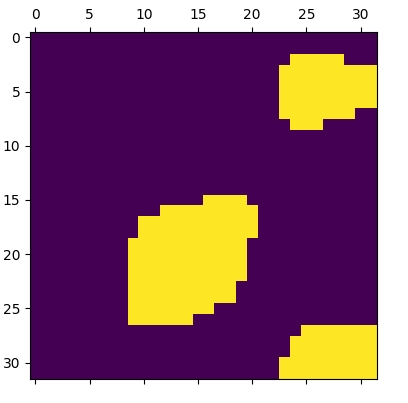
\includegraphics[width=0.196\textwidth]{fig/cae_gen.jpg}}
	\end{center}
	\vspace{-4mm}
	\caption{The input and output of the trained Convolutional Autoencoder on a test image.}
	\label{fig:2}
	\vspace{-0mm}
\end{figure}

\begin{figure}[h!]
	\begin{center}
		\subfigure[Input \label{fig:3a}]{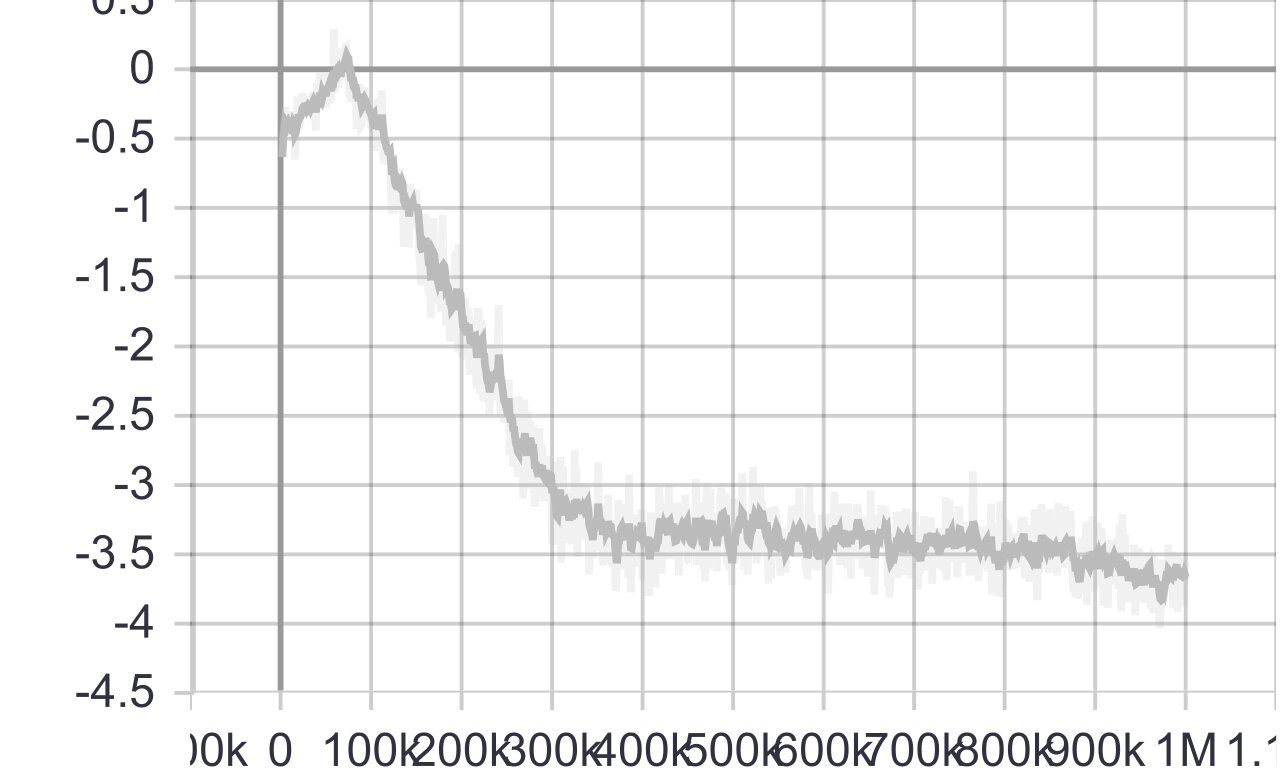
\includegraphics[width=0.2\textwidth]{fig/DDPG_actor_loss.jpg}}
		~
		\subfigure[Output \label{fig:3b}]{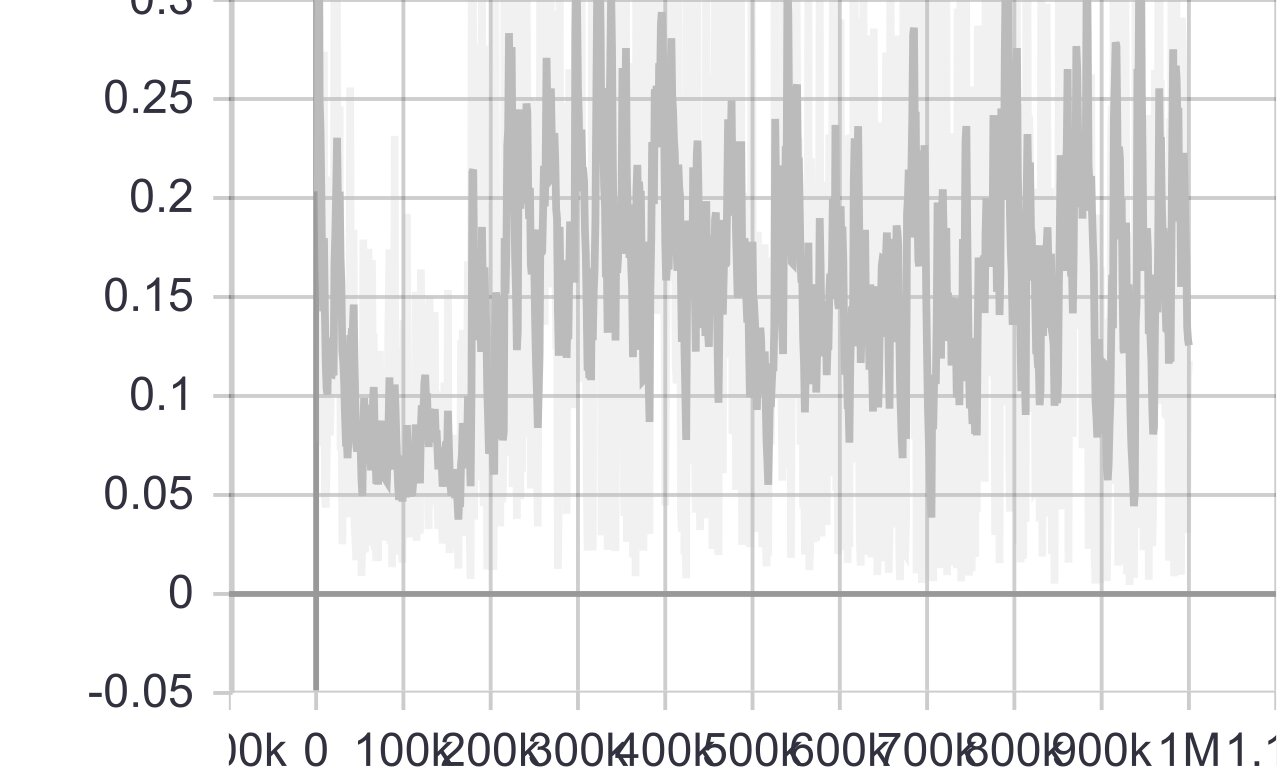
\includegraphics[width=0.2\textwidth]{fig/DDPG_critic_loss.jpg}}
	\end{center}
	\vspace{-4mm}
	\caption{The input and output of the trained Convolutional Autoencoder on a test image.}
	\label{fig:3}
	\vspace{-0mm}
\end{figure}

\begin{figure}[h!]
	\begin{center}
		\subfigure[Input \label{fig:4a}]{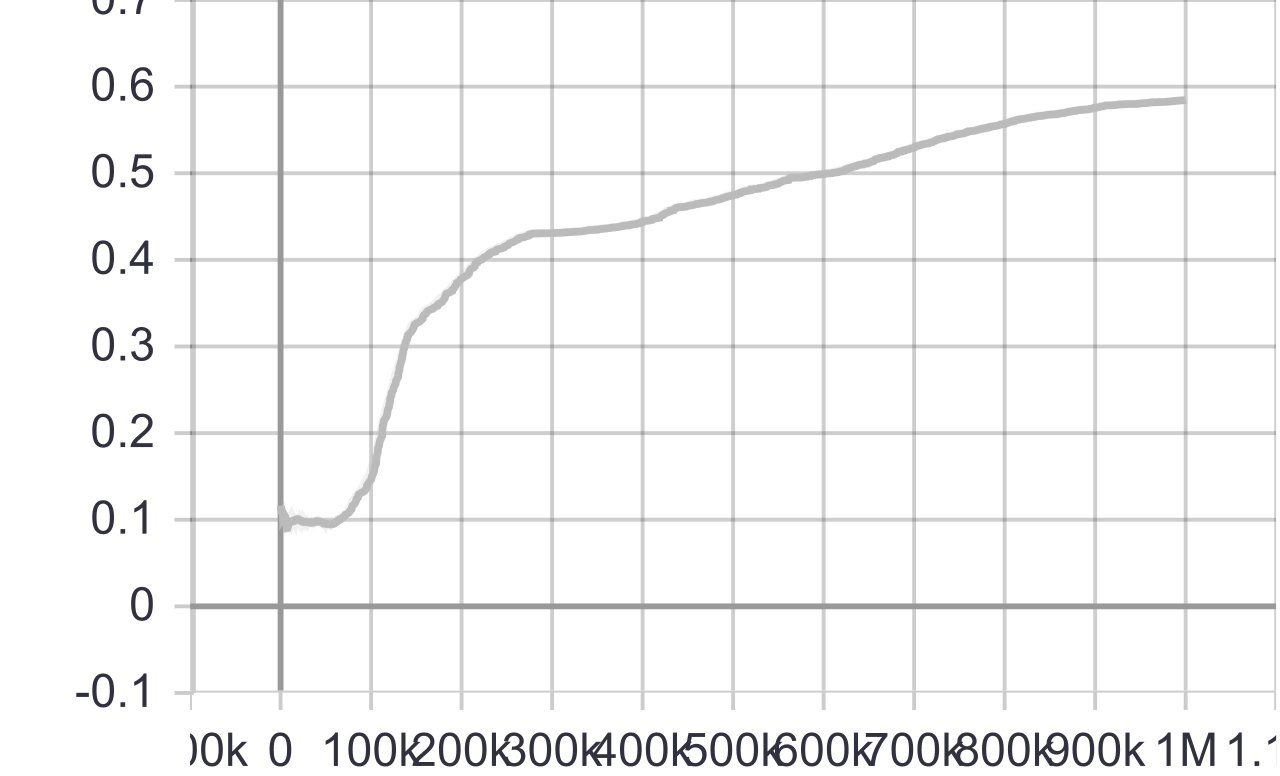
\includegraphics[width=0.2\textwidth]{fig/Common_training_success_rate.jpg}}
		~
		\subfigure[Output \label{fig:4b}]{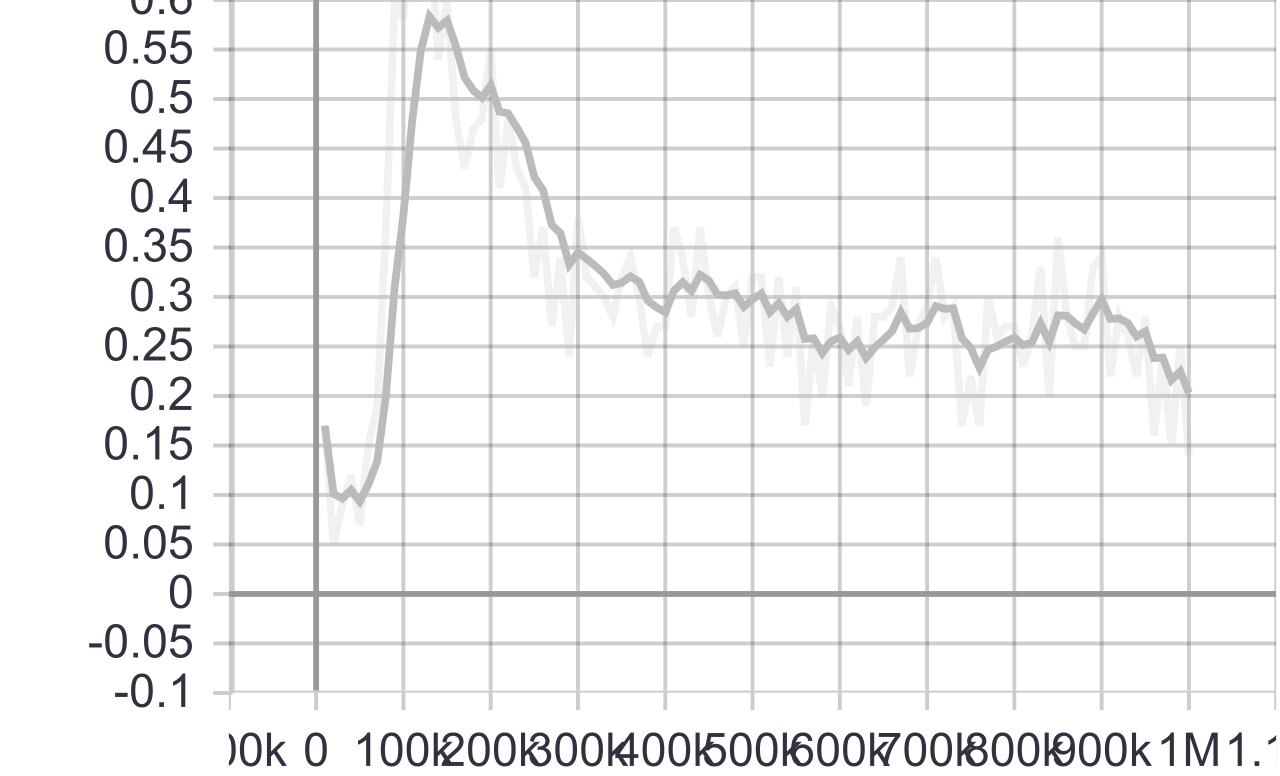
\includegraphics[width=0.2\textwidth]{fig/Common_test_success_rate.jpg}}
	\end{center}
	\vspace{-4mm}
	\caption{The input and output of the trained Convolutional Autoencoder on a test image.}
	\label{fig:4}
	\vspace{-0mm}
\end{figure}



\section{Future work}

As it was said previously, the next step is to find the good hyperparameters for training. If we managed to train the agent sufficiently, we will evaluate the results. We have in mind to compare the trained agents performance to a benchmark agent. For the benchmark agent, the reasonable choices would be for example a DDPG agent without HER and the agent that was trained with the method explained in \cite{NMP}.

If there will be enough time remaining, we will experiment with more sophisticated relabeling methods and possibly try to apply the whole method to a more complex robot, for example to a robot arm.


\bibliographystyle{IEEEtran}
\bibliography{bib/references.bib}
		
\end{document}